\begin{figure}[thb]
    \begin{center}
        \begin{minipage}{1.0\hsize}
            \begin{center}
            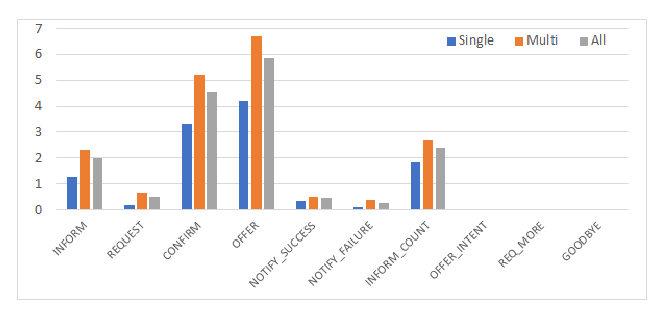
\includegraphics[clip, width=14cm]{chapter5/kouhoslot.eps}
            \caption{1対話あたりの各対話行為の発話中でスロット値候補が出現した回数}
            \label{fig:kouhoslot}
            \hspace{1.6cm}
            \end{center}
        \end{minipage}
        \begin{minipage}{1.0\hsize}
            \begin{center}
            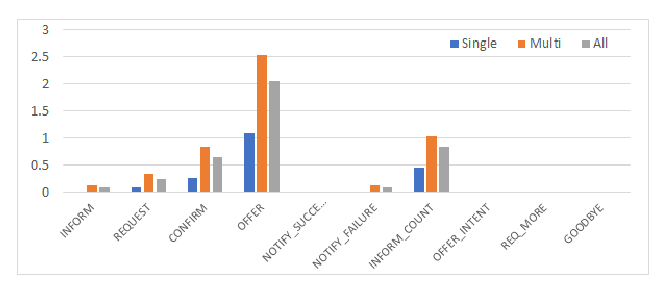
\includegraphics[clip, width=14cm]{chapter5/updateslot.eps}
            \caption{1対話あたりの各対話行為の発話中で出現したスロット値候補が実際にスロット値に反映された回数}
            \label{fig:updateslot}
            \end{center}
        \end{minipage}
    \end{center}
\end{figure}

結果は図\ref{fig:kouhoslot}と図\ref{fig:updateslot}に示す.この図では,Single-domain, Multi-domain,加えてその 2 つを合わせた All で結果に差異がないか調べるためにデータを分けて3つの結果を示している.図\ref{fig:kouhoslot}を見ると,“INFORM”と“CONFIRM”, “OFFER”, “INFORM\_COUNT”では他の対話行為に比べて多くのスロット値候補が出現していることが分かる.“INFORM”,“CONFIRM”,“OFFER”は,スロット値に関する発話を行うため,スロット値候補が多く出現している.ただし,“INFORM\_COUNT”はユーザの要求に合致する対象の個数を通知する対話行為であるため,それ自体がスロット値候補を与えることはないが,“OFFER”と同じ発話で共存していることが多い.そのため,“INFORM\_COUNT”の発話でもスロット値候補が多く出現している.残りの対話行為は,スロット値に関する発話を行わなず,他の対話行為と共存することも少ないため,発話中にスロット値候補が出現することが少ない.
\par
図\ref{fig:updateslot}を見ると,“INFORM”と“CONFIRM”は出現したスロット値候補に対して約10分の1しか対話状態に反映されていないことが分かる.これは両者ともに対話状態の更新に必要でないスロット値候補を多く与えているからである.例えば,“INFORM”が与えるスロット値候補はユーザが指定したものや場所の補足情報であり,対話状態を更新する情報ではないことが多い.また,“CONFIRM”の発話は既に対話状態に含まれているスロット値の確認を行うため,与えるスロット値候補の多くは既に対話状態に反映されており,対話状態が更新されない.ただし,“CONFIRM”が与えるスロット値候補は,ユーザが発した単語の言い換え(例:“at afternoon 1:30” $\rightarrow$ “1:30 pm”)を含むため対話状態にスロット値として追加されることもある.反対に,“OFFER”と“INFORM\_COUNT”は与えたスロット値候補の約4分の1が対話状態に反映されていることが分かる.したがって,両者どちらかの対話行為タグを持つ発話で出現するスロット値候補は対話状態に反映される可能性が高く,その発話は他の対話行為の発話よりスロット値の推定に重要であると考えられる.ただし,“CONFIRM”の説明で述べたように,対話行為ごとに与える情報に特徴があるため,一概に“OFFER”と“INFORM\_COUNT”を持つ発話だけが重要とは言えない.また,以上に示した結果は Single-domain, Multi-domain,加えてその 2 つを合わせた All でも同様の結果となっている.